\begin{figure}[h!]
    \centering
    \caption{Changes in MW measures in Chicago on July 2019}
    \label{fig:map_mw_chicago_jul2019}

    \begin{subfigure}{0.5\textwidth}
        \centering
        \caption{Residence MW}
        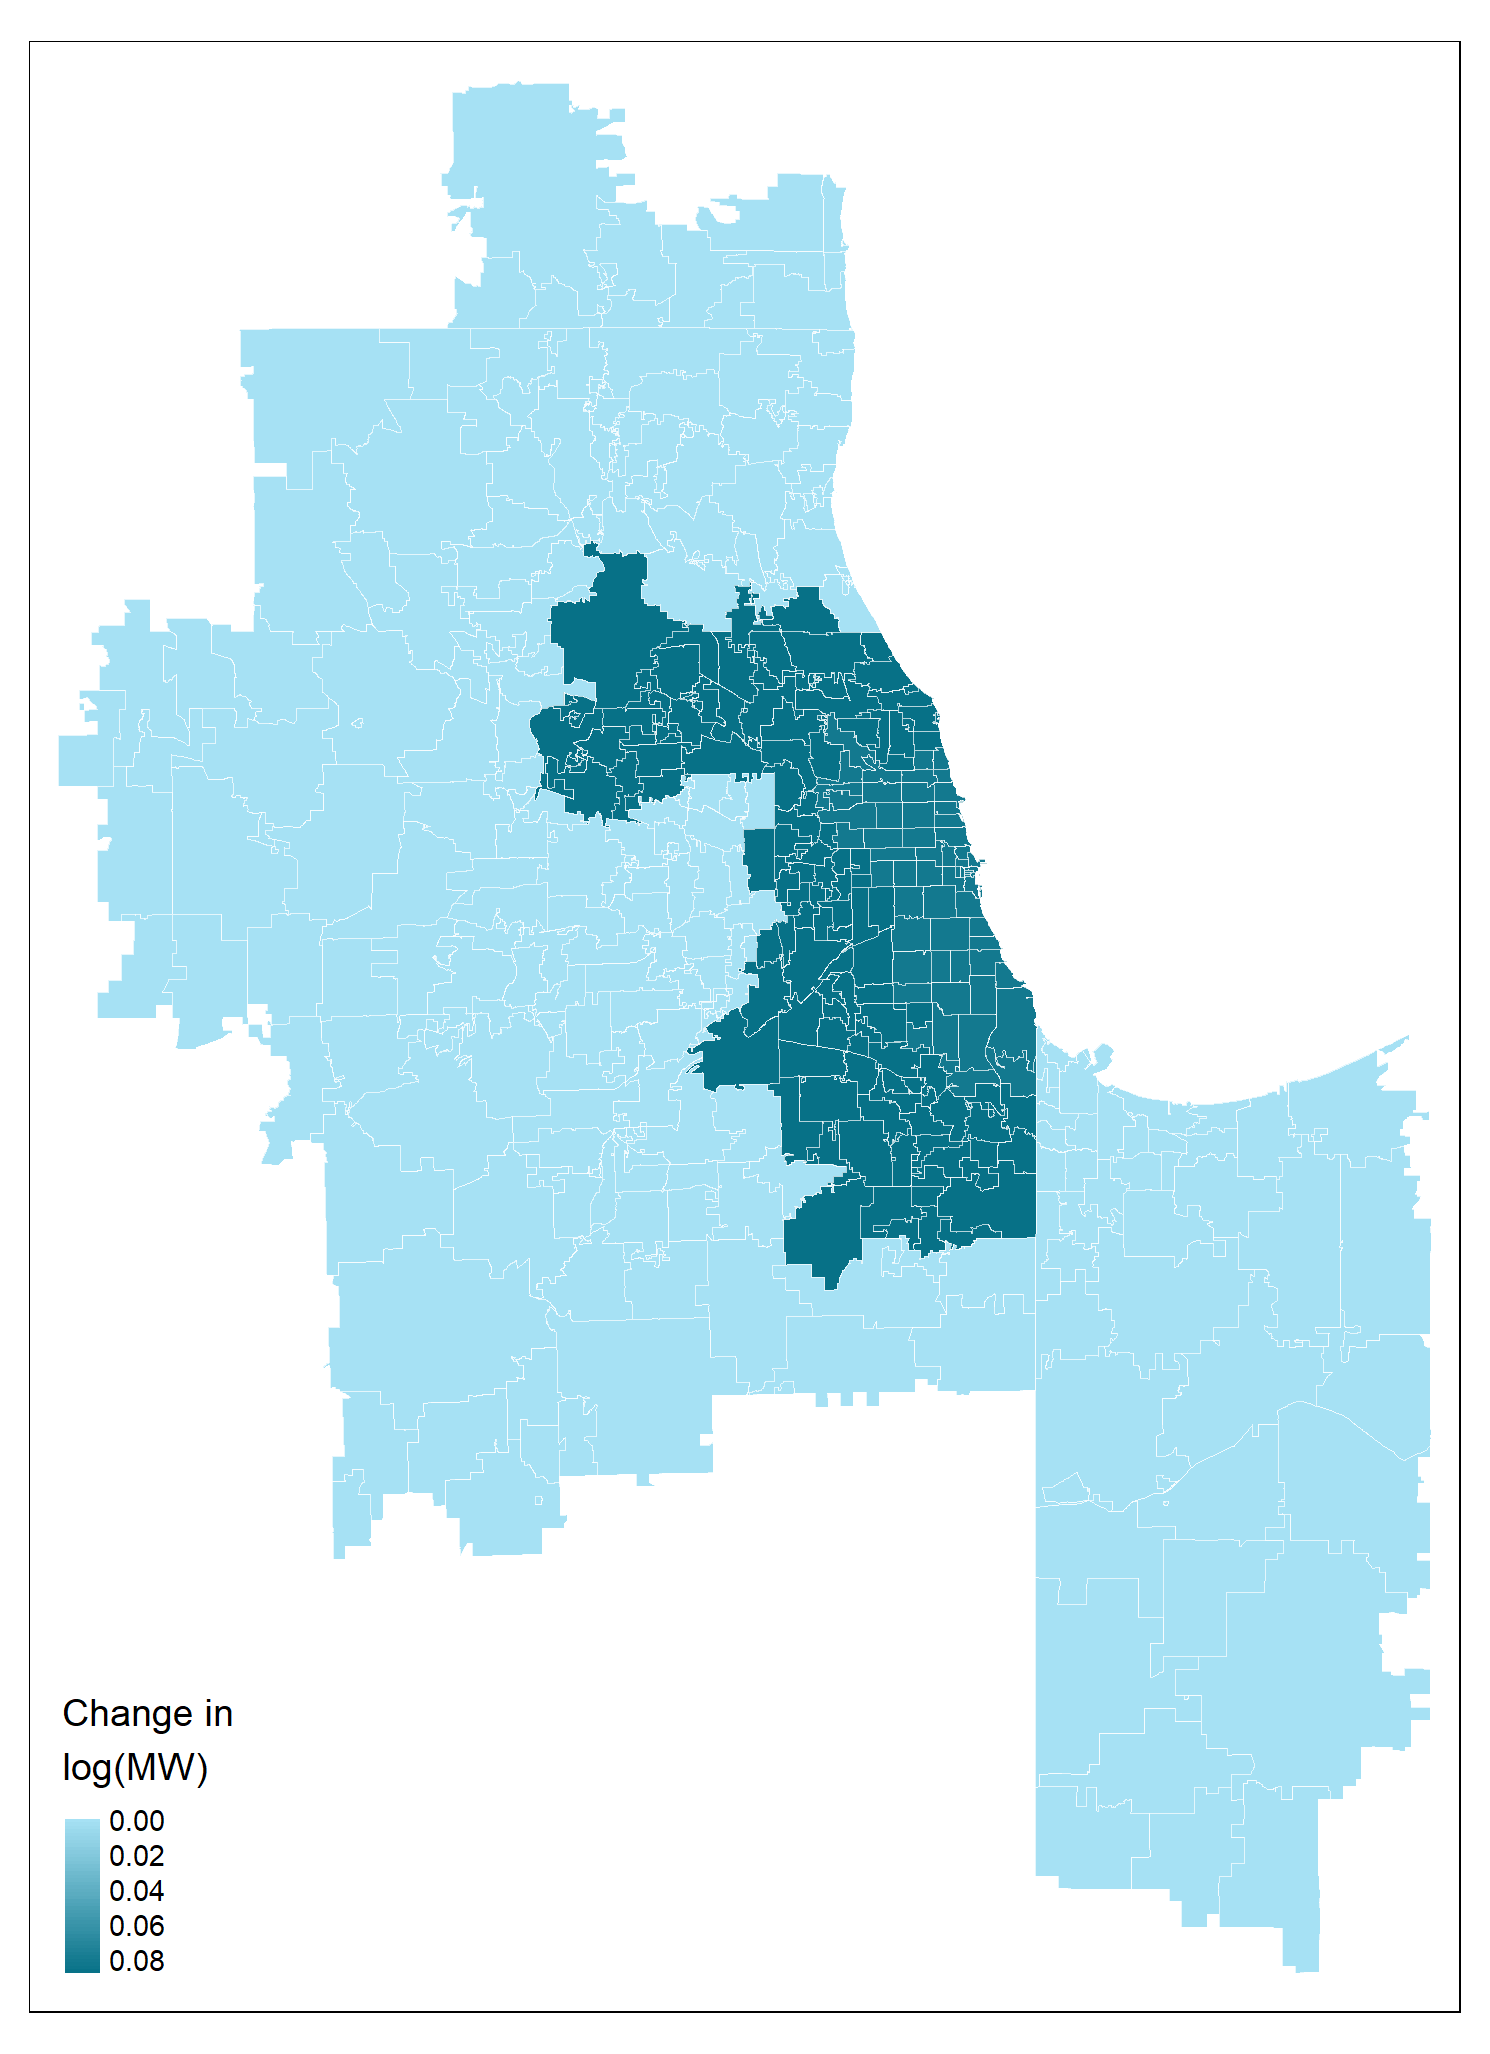
\includegraphics[width = 1\textwidth]
            {maps_events/output/chicago_2019-6_actual_mw.png}
    \end{subfigure}%
    \begin{subfigure}{0.5\textwidth}
        \centering
        \caption{Workplace MW}
        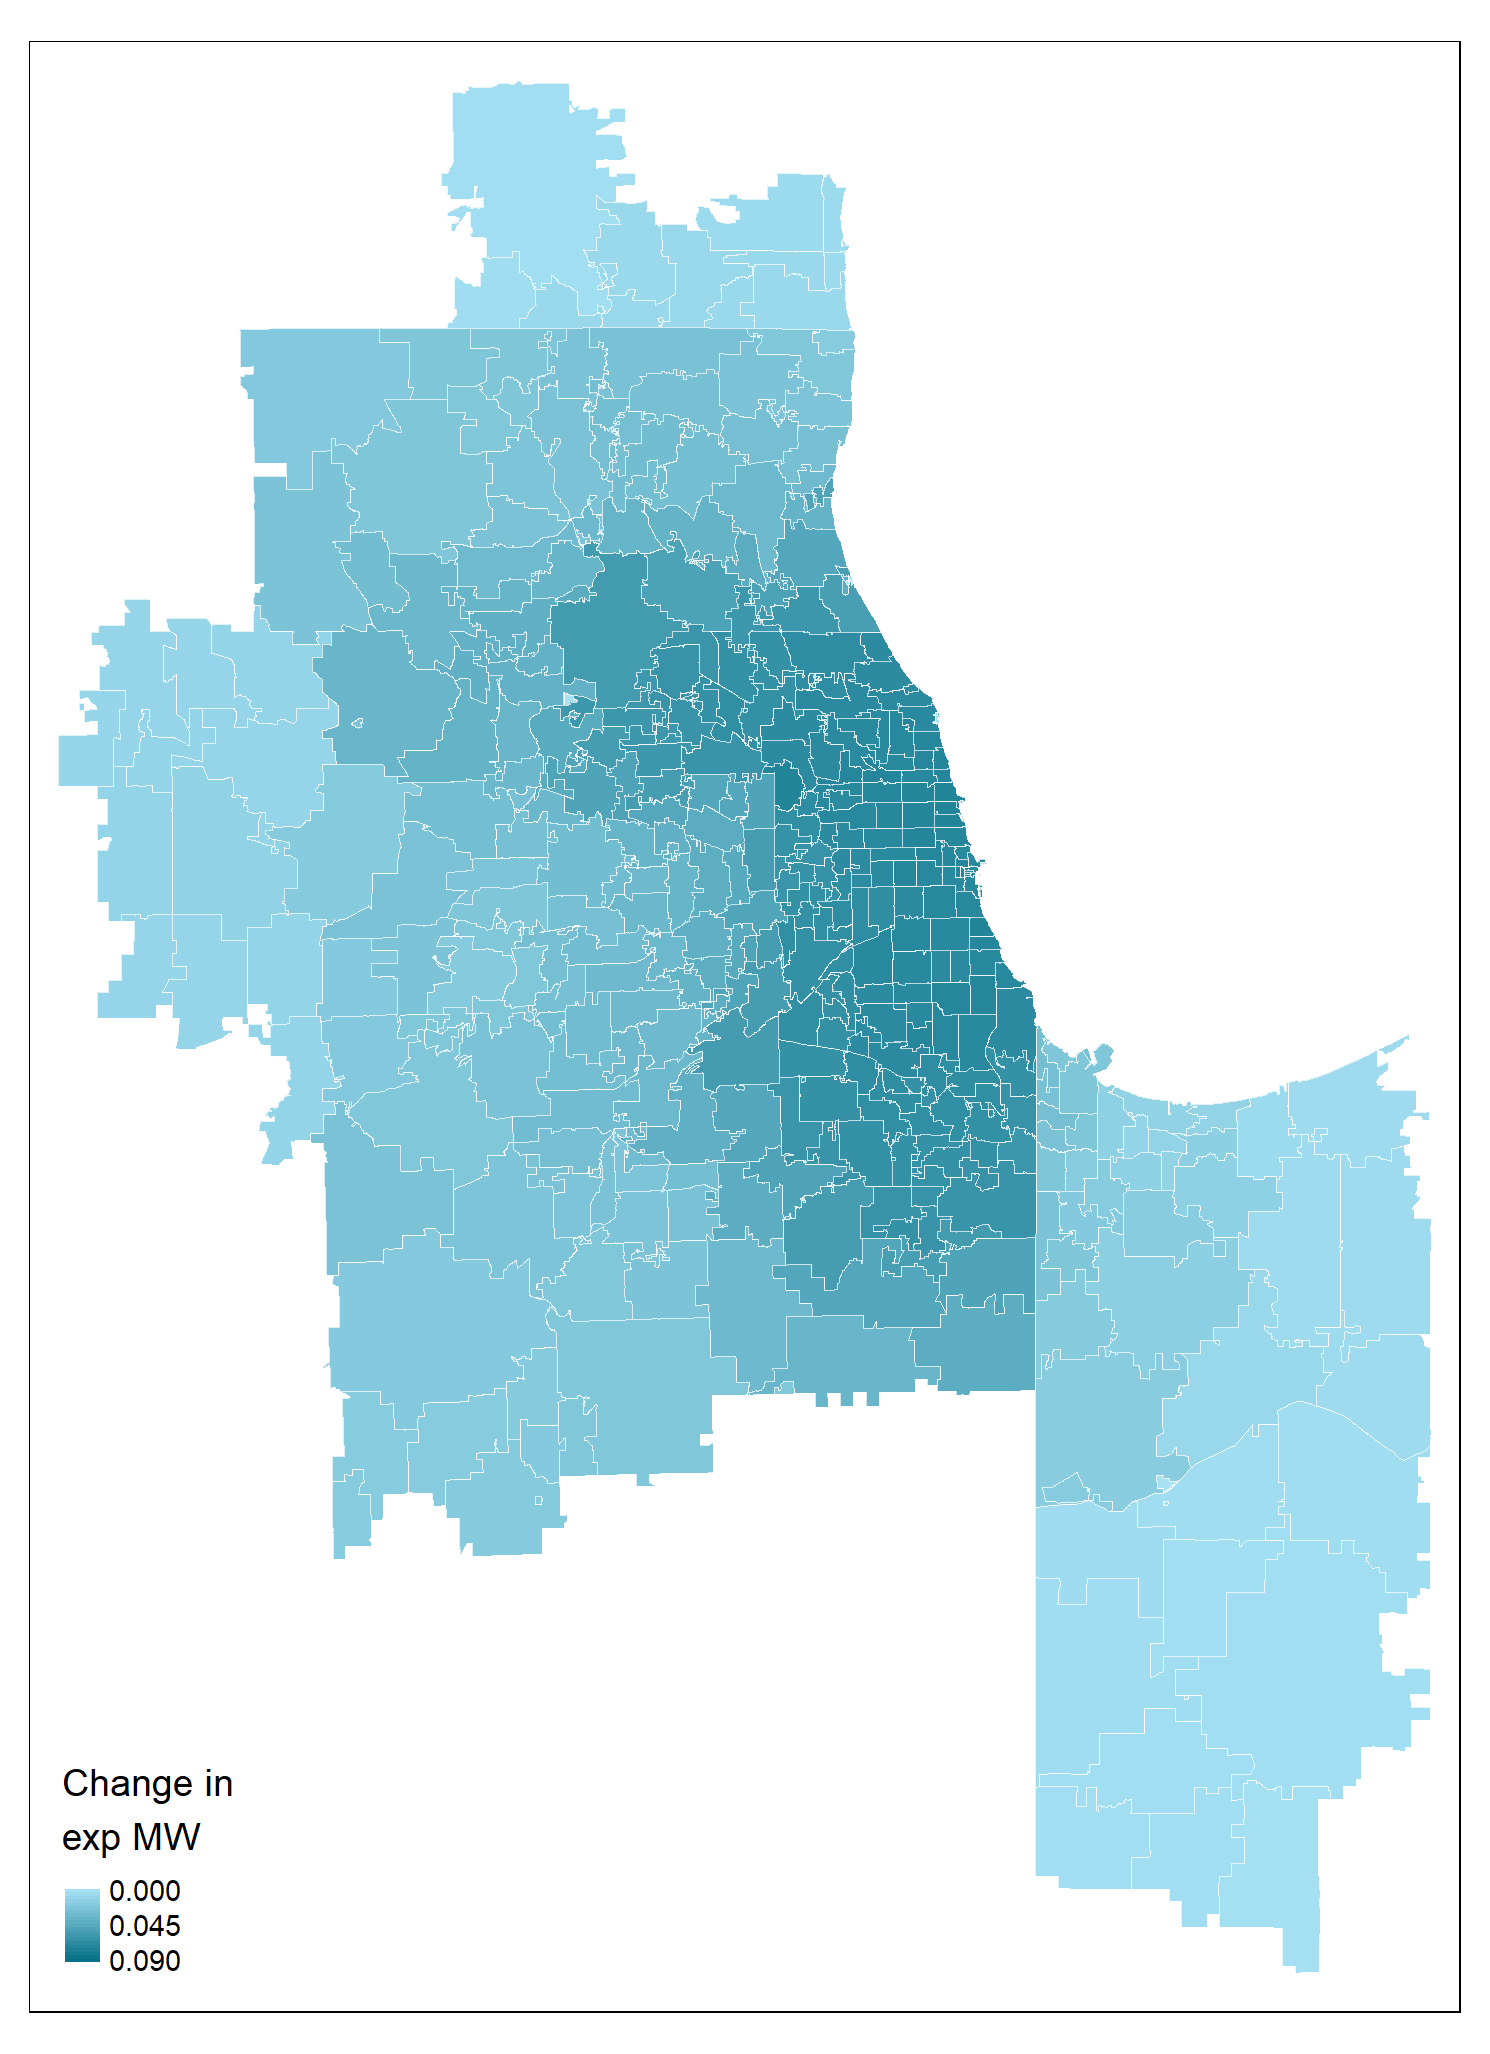
\includegraphics[width = 1\textwidth]
            {maps_events/output/chicago2019-6_exp_mw.png}
    \end{subfigure}

    %%
    %% SH: Some comments on the plots
    %%     - Can we drop the boxes around the maps?
    %%     - Can we change legends to 'Change in\nresidence MW'
    %%                            and 'CHange in\nworkplace MW'?
    %%

    \begin{minipage}{.95\textwidth} \footnotesize
        \vspace{3mm}
        Notes: 
        Data are from the MW panel defined in Section 
        \label{sec:mw_construction} and from LODES \parencite{LODES}.
        The figure shows the change in 
        the residence MW (panel a) and workplace MW (panel b) 
        on July 2019 in the metropolitan area of Chicago.
        The residence MW is defined as the log of the statutory MW of the given
        ZIP code.
        The workplace MW is defined as the weighted average of the log of the
        statutory MW levels in workplace locations of a ZIP code's residents,
        where weights are given by commuting shares.
    \end{minipage}
\end{figure}
